
\chapter{Sorting Algorithms}

\section{RAM Model}

\subsection{Characteristics}

\subsubsection*{Comparison-based vs Non-comparison-based}

\begin{itemize}
    \item \textbf{Comparison-based} algorithms are algorithms that sort a list by comparing elements of the list. These algorithms generally have lower bounds of O(n log n). The most common comparison-based sorting algorithms are:
    \begin{itemize}
        \item Bubble Sort
        \item Selection Sort
        \item Insertion Sort
        \item Merge Sort
        \item Quick Sort
        \item Heap Sort
    \end{itemize}
    \item \textbf{Non-comparison-based} don’t rely on comparisons but instead use counting, hashing, or other methods to determine the order. They can sometimes achieve better time complexity (e.g., O(n)). The most common non-comparison-based sorting algorithms are:
    \begin{itemize}
        \item Counting Sort
        \item Radix Sort
        \item Bucket Sort
    \end{itemize}
\end{itemize}

\subsubsection*{Space Complexity}

How much extra memory is required by the algorithm relative to the size of the input. For example, an algorithm that requires O(n) extra space is less efficient in terms of memory usage than one that requires only O(1) space.

\subsubsection*{Stability}

A sorting algorithm is \textbf{stable} if it preserves the relative order of records with equal keys (i.e., elements that compare equal will retain their original order). The most common stable sorting algorithms are:
\begin{itemize}
    \item Bubble Sort
    \item Insertion Sort
    \item Merge Sort
\end{itemize}

\subsubsection*{In-place vs Out-of-place}

\begin{itemize}
    \item \textbf{In-place}: The algorithm sorts the elements by modifying the input array directly, using only a constant amount of extra space (O(1) space complexity). The most common in-place sorting algorithms are:
    \begin{itemize}
        \item Bubble Sort
        \item Selection Sort
        \item Insertion Sort
        \item Quick Sort
        \item Heap Sort
    \end{itemize}
    \item \textbf{Out-of-place}: The algorithm requires additional space to hold a separate copy of the data (e.g., merge sort uses extra space for merging).
\end{itemize}

\subsubsection*{Online vs Offline}

\begin{itemize}
    \item \textbf{Online}: These algorithms can process the input in a piece-by-piece manner without needing the entire dataset upfront (e.g., insertion sort).
    \item \textbf{Offline}: These algorithms require the entire dataset to be available before they can start sorting (e.g., merge sort).
\end{itemize}

\subsubsection*{Divide and Conquer}

Algorithms that use the divide-and-conquer paradigm divide the problem into smaller subproblems, solve each subproblem recursively, and then combine the results (e.g., merge sort, quicksort).
\begin{itemize}
    \item \textbf{Divide}: The algorithm divides the input into smaller subproblems.
    \item \textbf{Conquer}: The algorithm solves the subproblems recursively.
    \item \textbf{Combine}: The algorithm combines the solutions of the subproblems to solve the original problem.
\end{itemize}

\subsubsection*{Parallelism}

Some sorting algorithms can take advantage of parallelism to speed up the sorting process. For example, merge sort can be parallelized by dividing the input into smaller subproblems and sorting them in parallel.

\subsubsection*{Recursive vs Iterative}

\begin{itemize}
    \item \textbf{Recursive}: Algorithms like quicksort and merge sort use recursion to break down the problem into smaller subproblems.
    \item \textbf{Iterative}: Algorithms like bubble sort and insertion sort use loops and iteration to solve the problem without recursion.
\end{itemize}


\newpage

\subsection{Insertion Sort}

\begin{algorithm}[H]
    \caption{Insertion Sort (A)}
    \For{j=2 to n}{
        key = A[j]\; \tcp*{$1\times (n-1)$}
        i = j - 1\; \tcp*{$1\times (n-1)$}
        \While{i > 0 and A[i] > key}{ 
            A[i + 1] = A[i]\; \tcp*{$1\times \frac{n(n-1)}{2}$}
            i = i - 1\; \tcp*{$1\times \frac{n(n-1)}{2}$}
        }
        A[i + 1] = key\;\tcp*{$1\times (n-1)$}
    }
\end{algorithm}

\begin{itemize}
    \item \textbf{Best case}: \theta($n$)
    \item \textbf{Worst case}: \theta($n^2$)
\end{itemize}

\definitionblock[Insertion Sort]{The basic concept of the Insertion Sort algorithm is to build a sorted array (or list) one element at a time by repeatedly taking the next element from the unsorted portion and inserting it into the correct position within the sorted portion. This process is similar to how one might sort playing cards in their hands.}
Here's a step-by-step explanation:

\begin{itemize}
    \item Start with the second element (index 1) of the array. This element is considered the "key" and will be compared with the elements before it.
    \item Compare the key with the element before it. If the key is smaller, shift the previous element to the right.
    \item Continue shifting elements to the right until you find the correct position for the key.
    \item Insert the key into its correct position.
    \item Move to the next element and repeat the process until the entire array is sorted.
\end{itemize}

\begin{figure}[H]
    \centering
    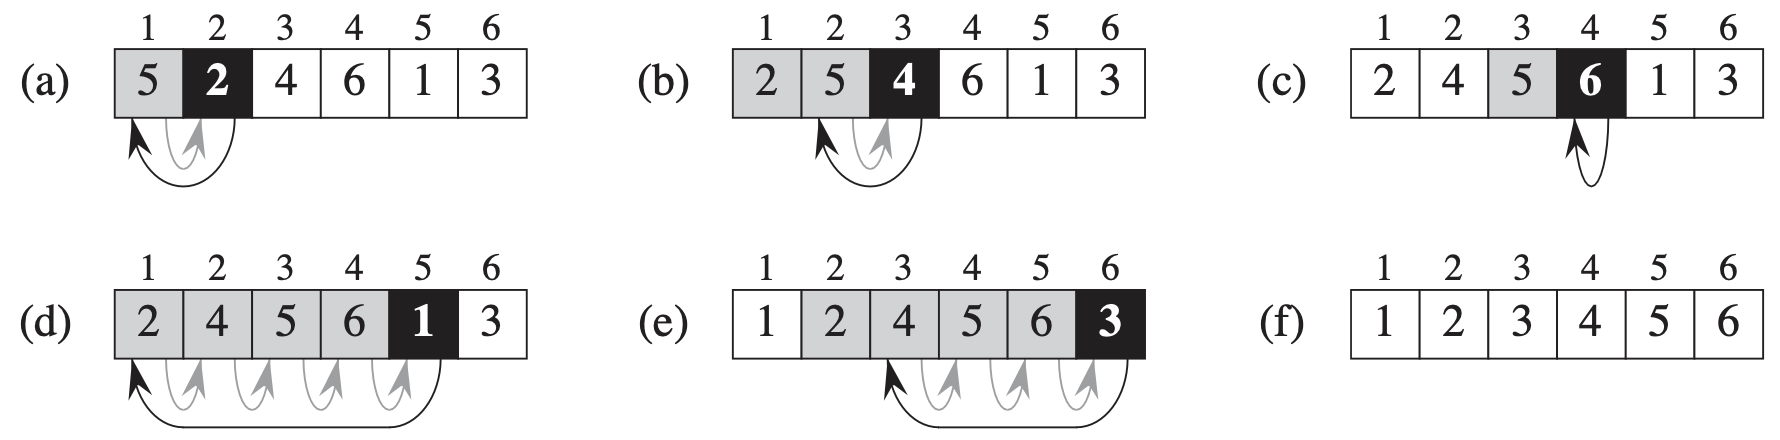
\includegraphics[width=0.8\textwidth]{assets/insertion_sort.png}
    \caption{Insertion Sort (\cite{cormen2022introduction})}
\end{figure}

\subsubsection*{Characteristics}

\begin{itemize}
    \item \textbf{Stable}: Yes
    \item \textbf{In-place}: Yes
    \item \textbf{Online}: Yes
    \item \textbf{Divide and Conquer}: No
    \item \textbf{Parallelism}: No
    \item \textbf{Recursive vs Iterative}: Iterative
    \item \textbf{Space Complexity}: O(1)
    \item \textbf{Comparison-based}: Yes
\end{itemize}

\newpage

\subsection{Merge Sort}

\begin{algorithm}[H]
    \caption{Merge Sort (A, p, r)}
    \If{p < r}{
        q = $\lfloor \frac{p + r}{2} \rfloor$\;
        MergeSort(A, p, q)\; \tcp*{Recursively sort the left half}
        MergeSort(A, q + 1, r)\; \tcp*{Recursively sort the right half}
        Merge(A, p, q, r)\; \tcp*{Merge the two sorted halves}
    }
    \tcc{$1+log{n}$ levels of the tree structure}
    \tcc{Time complexity: $\theta(n \log n)$}
\end{algorithm}

The MERGE-SORT procedure splits the array into two halves, recursively sorts each half, and then merges the two sorted halves. The base case of the recursion occurs when the array to be sorted has length 1, in which case there is no work to be done, since every array of length 1 is already sorted. 
\observationblock[Stopping condition]{It stops when there is one element in the array, where $p=r$.}
\begin{algorithm}[H]
    \caption{Merge (A, p, q, r)}
    $n_1 = q-p+1$\;
    $n_2 = r-q$\;
    \tcc{Copy the new portions of the array into two new arrays\;}
    \For{i=1 to n1}{
        L[i] = A[p+i-1]\;
    }
    \For{j=1 to n2}{
        R[j] = A[q+j]\;
    }
    L[n1+1] = $\infty$\;
    R[n2+1] = $\infty$\;
    i = 1\;
    j = 1\;
    \tcc{Two-fingers merge algorighm\;}
    \For{k=p to r}{
        \If{L[i] $\leq$ R[j]}{
            A[k] = L[i]\;
            i = i + 1\;
        }
        \Else{
            A[k] = R[j]\;
            j = j + 1\;
        }
    }
    \tcc{Time complexity: $\theta(n)$}
\end{algorithm}

\definitionblock[Merge Sort]{This algorithm is a \textbf{divide-and-conquer} algorithm that divides the input array into two halves, recursively sorts the two halves, and then merges the sorted halves. The merge operation combines two sorted arrays into a single sorted array. It is also \textbf{recursive} in its structure since it calls itself on subproblems.}

The recursion “bottoms out” when the sequence to be sorted has length 1, in which
case there is no work to be done, since every sequence of length 1 is already in
sorted order.
The key operation of the merge sort algorithm is the merging of two sorted
sequences in the “combine” step. We merge by calling an auxiliary procedure
$MERGE(A,p,q,r)$, where A is an array and p, q, and r are indices into the array
such that $p \leq q < r$. The procedure assumes that the subarrays $A[p\dots q]$ and
$A[q+1 \dots r]$ are in sorted order. It merges them to form a single sorted subarray
that replaces the current subarray $A[p \dots r]$.

\begin{center}
    \begin{figure}[H]
        \centering
        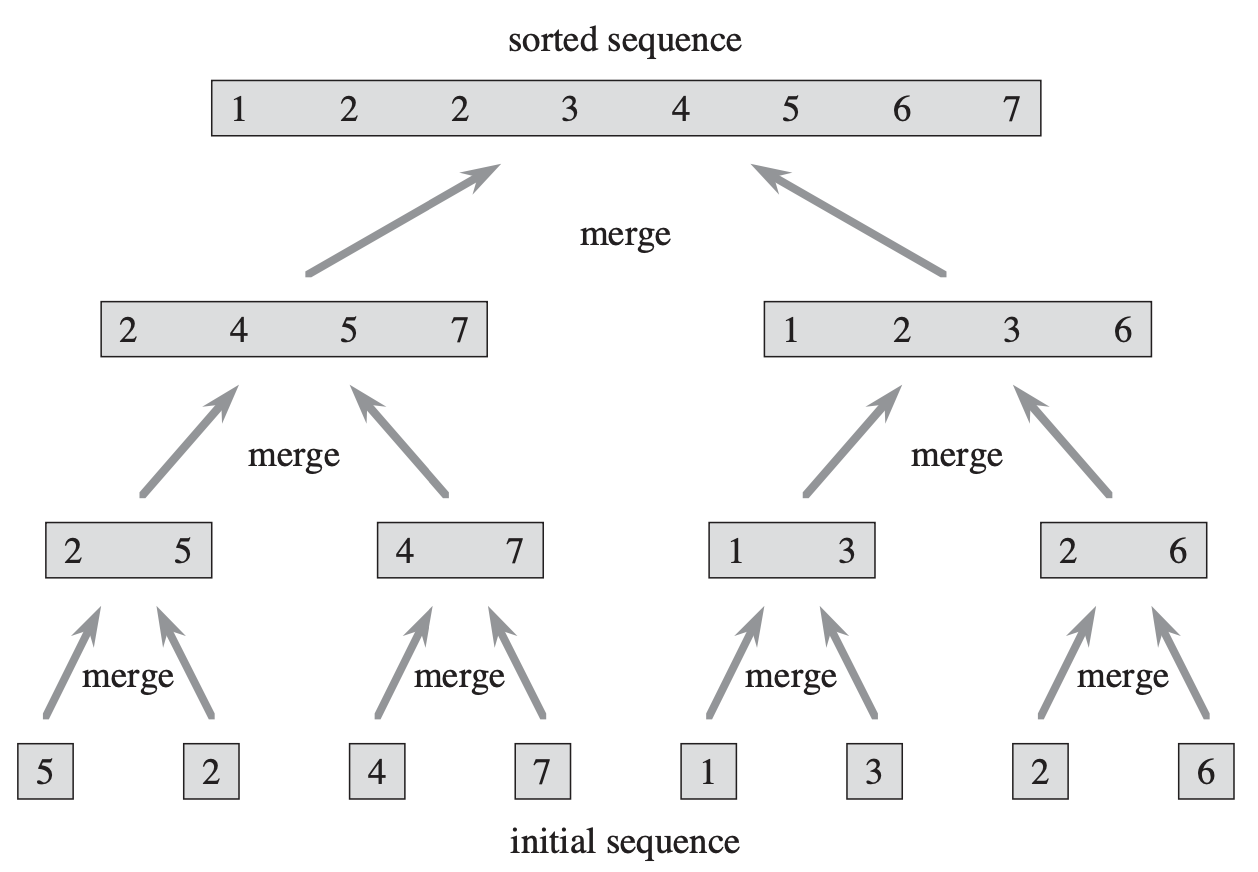
\includegraphics[width=0.7\textwidth]{assets/merge_sort.png}
        \caption{Merge Sort (\cite{cormen2022introduction})}
    \end{figure}
\end{center}

\subsubsection*{Time complexity analysis}

We reason as follows to set up the recurrence for T .n/, the worst-case running
time of merge sort on n numbers. Merge sort on just one element takes constant
time. When we have $n > 1$ elements, we break down the running time as follows.
\begin{itemize}
    \item \textbf{Divide}: The divide step just computes the middle of the subarray, which takes constant time. Thus, $D(n) = \theta(1)$.
    \item \textbf{Conquer}: We recursively solve two subproblems, each of size $n=2$, which contributes $2T(n/2)$ to the running time.
    \item \textbf{Combine}: The MERGE procedure on a subarray of size n takes time $\theta(n)$, and so $C(n) = \theta(n)$.
\end{itemize}

Where 

\begin{center}
    $T(n) = \begin{cases} 
        \theta(1) & \text{if $n = 1$} \\
        2T(n/2) + \theta(n) & \text{if $n > 1$}
    \end{cases}$
\end{center}

And the solution to this recurrence is $T(n) = \theta(n \log n)$.

\subsubsection*{Characteristics}

\begin{itemize}
    \item \textbf{Stable}: Yes
    \item \textbf{In-place}: No
    \item \textbf{Online}: No
    \item \textbf{Divide and Conquer}: Yes
    \item \textbf{Parallelism}: Yes
    \item \textbf{Recursive vs Iterative}: Recursive
    \item \textbf{Space Complexity}: O(n)
    \item \textbf{Comparison-based}: Yes
\end{itemize}



\subsection{Heapsort}

The \textbf{(binary) heap} data structure is an array object that we can view as a nearly complete binary tree. Each node of the tree corresponds to an element of the array. The tree is completely filled on all levels except possibly the lowest, which is filled from the left up to a point.

\begin{figure}[H]
    \centering
    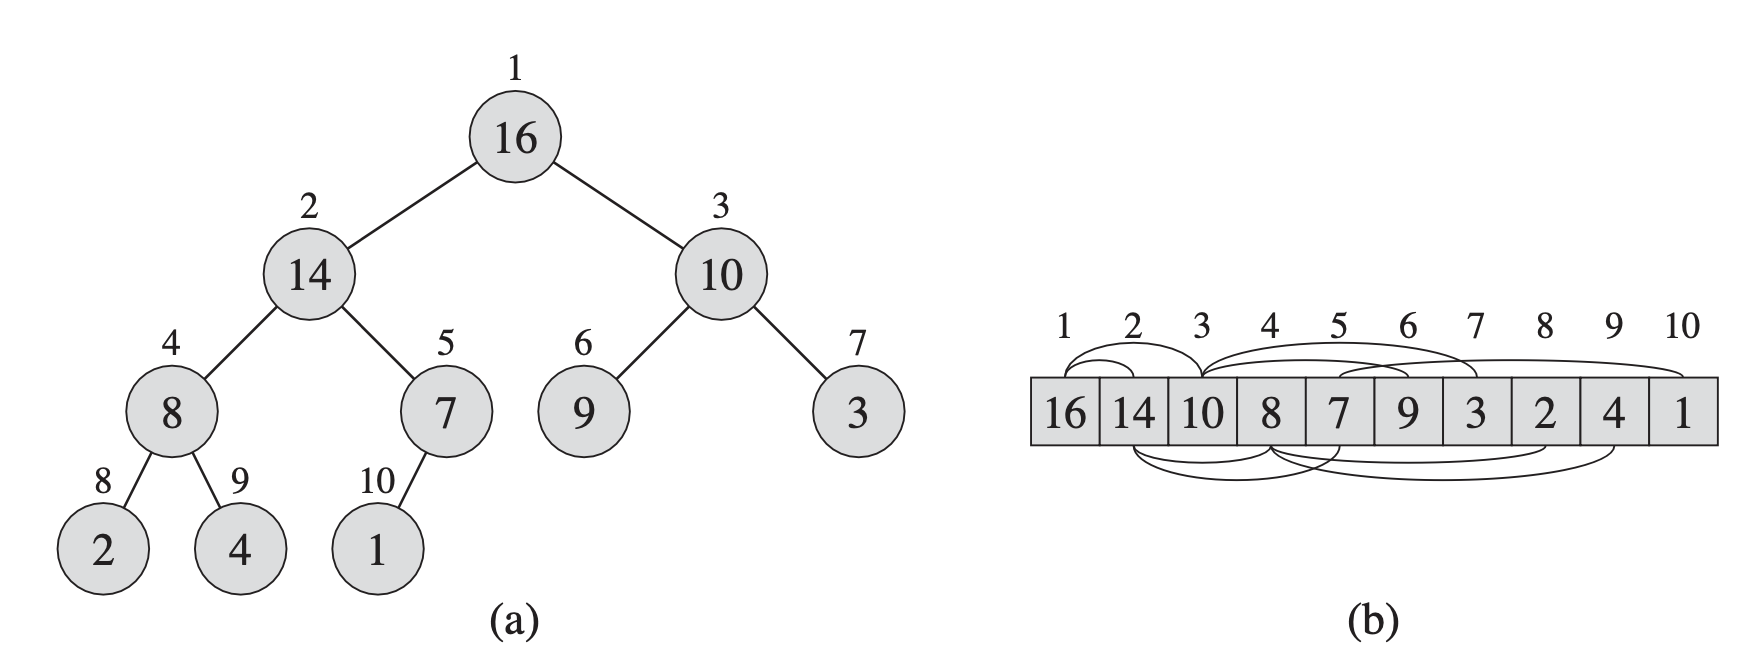
\includegraphics[width=0.7\textwidth]{assets/heap.png}
    \caption{A max-heap viewed as a Binary Tree (a) and an array (b) (\cite{cormen2022introduction})}
\end{figure}

The root of the tree is $A[1]$ , and given the index i of a node, we
can easily compute the indices of its parent, left child, and right child:

\begin{itemize}
    \item \textbf{Parent}: $\lfloor i/2 \rfloor$
    \item \textbf{Left child}: $2i$
    \item \textbf{Right child}: $2i + 1$
\end{itemize}

There are two kinds of binary heaps: max-heaps and min-heaps. In both kinds,
the values in the nodes satisfy a \textbf{heap property}, the specifics of which depend on
the kind of heap.

\definitionblock[Max-heap property]{The \textbf{max-heap property} is that for every node i other than the root, $A[PARENT(i)] \geq A[i]$. That is, the value of a node is at most the value of its parent.}
\definitionblock[Min-heap property]{The \textbf{min-heap property} is that for every node i other than the root, $A[PARENT(i)] \leq A[i]$. That is, the value of a node is at least the value of its parent.}

\begin{algorithm}[H]
    \caption{Max-Heapify (A, i)}
    l = LEFT(i)\;
    r = RIGHT(i)\;
    \If{l $\leq$ heap-size[A] and A[l] > A[i]}{
        largest = l\;
    }
    \Else{
        largest = i\;
    }
    \If{r $\leq$ heap-size[A] and A[r] > A[largest]}{
        largest = r\;
    }
    \If{largest $\neq$ i}{
        exchange A[i] with A[largest]\;
        Max-Heapify(A, largest)\;
    }
    \tcc{Levels: $\log n$}
    \tcc{Time complexity: $\theta(\log n)$}
\end{algorithm}

\begin{algorithm}[H]
    \caption{Build-Max-Heap (A)}
    heap-size[A] = length[A]\;
    \For{i = $\lfloor$ length[A]/2 $\rfloor$ downto 1}{
        Max-Heapify(A, i)\;
    }
    \tcc{Time complexity: $O(n\log n)$}
\end{algorithm}

\begin{algorithm}[H]
    \caption{Heap-Sort (A)}
    Build-Max-Heap(A)\; \tcp*{$O(n\log n)$}
    \For{i = length[A] downto 2}{ \tcp*{n times}
        exchange A[1] with A[i]\;
        heap-size[A] = heap-size[A] - 1\;
        Max-Heapify(A, 1)\; \tcp*{$O(\log n)$}
    }
    \tcc{Time complexity: $O(n\log n)$}
\end{algorithm}
\newpage

In order to maintain the max-heap property, we call the procedure MAX-HEAPIFY.
Its inputs are an array A and an index i into the array. When it is called, \textbf{MAX-
HEAPIFY assumes that the binary trees rooted at LEFT(i) and RIGHT(i) are max-
heaps}, but that A[i] might be smaller than its children, thus violating the max-heap
property. MAX-HEAPIFY lets the value at A[i] “float down” in the max-heap so
that the subtree rooted at index i obeys the max-heap property.

Note that:
\begin{itemize}
    \item \textbf{A.length} is the number of elements in the array.
    \item \textbf{A.heap-size} is the number of elements in the heap stored in array A.
\end{itemize}

\observationblock[Choosing i]{
    The procedure MAX-HEAPIFY is used in a bottom-up manner to convert an array A[1..n], where n = A.length, into a max-heap. The elements in the subarray A[$\lfloor n/2 \rfloor$+1..n] are all leaves of the tree, and so each is a 1-element heap to begin with. The procedure BUILD-MAX-HEAP goes through the remaining nodes of the tree and runs MAX-HEAPIFY on each one.
}

Viewing a heap as a tree, we define the height of a node in a heap to be the
number of edges on the longest simple downward path from the node to a leaf, and
we define the height of the heap to be the height of its root. Since a heap of $n$ elements is based on a complete binary tree, its height is $\theta(\log n)$.

We shall see that the basic operations on heaps run in time at most proportional
to the height of the tree and thus take $O(\log n)$ time.

\begin{figure}[H]
    \centering
    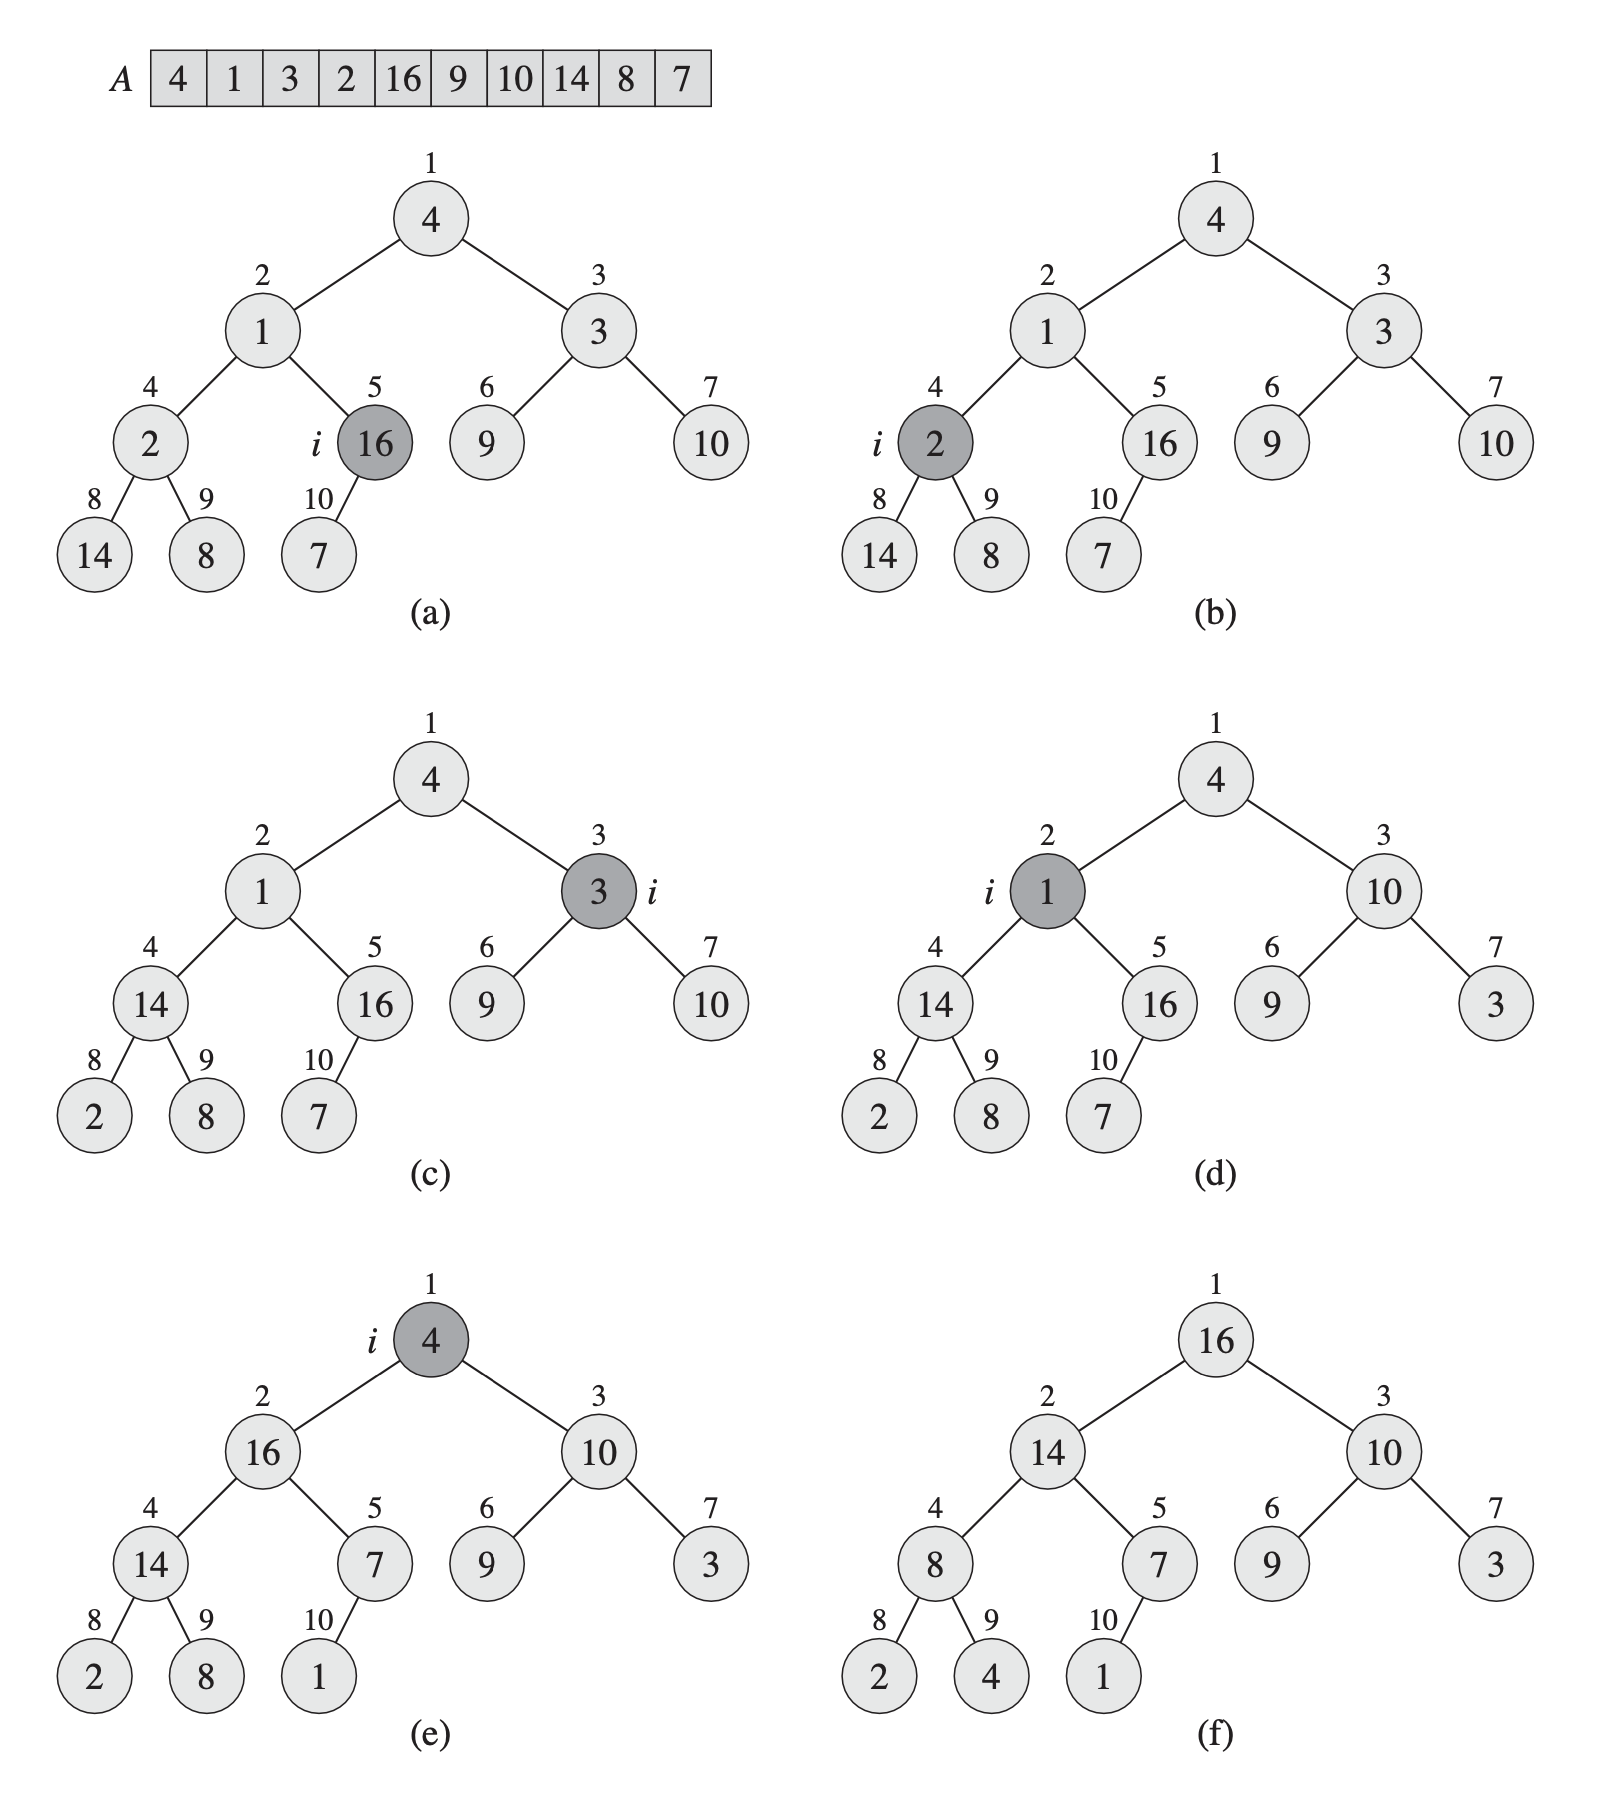
\includegraphics[width=0.6\textwidth]{assets/heapsort.png}
    \caption{BUILD-MAX-HEAP (\cite{cormen2022introduction})}
\end{figure}

\subsubsection*{Characteristics}

\begin{itemize}
    \item \textbf{Stable}: No
    \item \textbf{In-place}: Yes
    \item \textbf{Online}: No
    \item \textbf{Divide and Conquer}: No
    \item \textbf{Parallelism}: No
    \item \textbf{Recursive vs Iterative}: Recursive
    \item \textbf{Space Complexity}: O(1)
    \item \textbf{Comparison-based}: Yes
\end{itemize}


\subsection{Quicksort}

The quicksort algorithm has a worst-case running time of $\theta (n^2)$ on an input array
of n numbers. Despite this slow worst-case running time, quicksort is often the best
practical choice for sorting because it is remarkably efficient on the average: its
expected running time is $\theta (n\log n)$, and the constant factors hidden in the $\theta (n\log n)$
notation are quite small. It also has the advantage of sorting in place.

It uses the divide-and-conquer paradigm. Here is the basic idea:
\begin{itemize}
    \item \textbf{Divide}: Partition (rearrange) the array $A[p\dots r]$ into two (possibly empty) subar-
    rays $A[p\dots q-1]$ and $A[q+1\dots r]$ such that each element of $A[p\dots q-e]$ is
    less than or equal to A[q] , which is, in turn, less than or equal to each element
    of $A[q+1\dots r]$ . Compute the index q as part of this partitioning procedure.
    \item \textbf{Conquer}: Sort the two subarrays $A[p\dots q-1]$ and $A[q+1\dots r]$ by recursive calls to quicksort.
    \item \textbf{Combine}: Because the subarrays are already sorted, no work is needed to combine them: the entire array $A[p\dots r]$ is now sorted.
\end{itemize}

\begin{figure}[H]
    \centering
    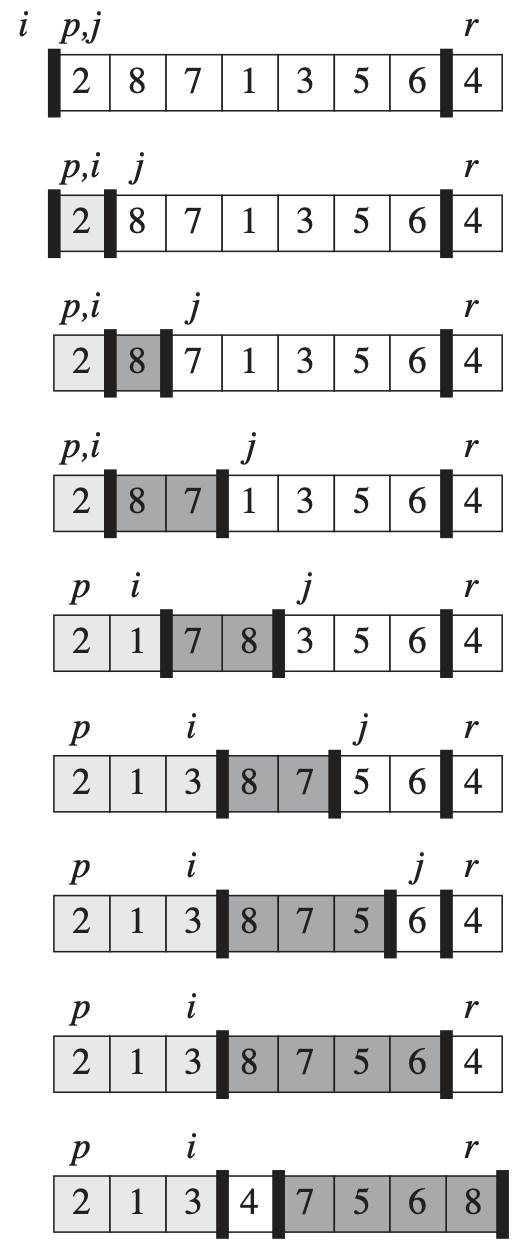
\includegraphics[width=0.15\textwidth]{assets/quicksort.png}
    \caption{Quicksort (\cite{cormen2022introduction})}
\end{figure}

\begin{algorithm}[H]
    \caption{Quicksort (A, p, r)}
    \If{p < r}{
        q = Partition(A, p, r)\;
        Quicksort(A, p, q-1)\;
        Quicksort(A, q+1, r)\;
    }
    \tcc{Worst case: $O(n^2)$, Average case: $O(n\log n)$}
\end{algorithm}

\begin{algorithm}[H]
    \caption{Partition (A, p, r)}
    x = A[r]\; \tcp*{Pivot element}
    i = p - 1\;
    \For{j = p to r-1}{
        \If{A[j] $\leq$ x}{
            i = i + 1\;
            exchange A[i] with A[j]\;
        }
    }
    exchange A[i+1] with A[r]\;
    \Return i + 1\;
    \tcc{Repeat n timess}
\end{algorithm}

\observationblock[i, j values]{
    The indices i and j are used to keep track of the elements in the array. The index i is used to keep track of the elements that are less than or equal to the pivot element, while the index j is used to iterate through the array.
}

\begin{figure}[H]
    \centering
    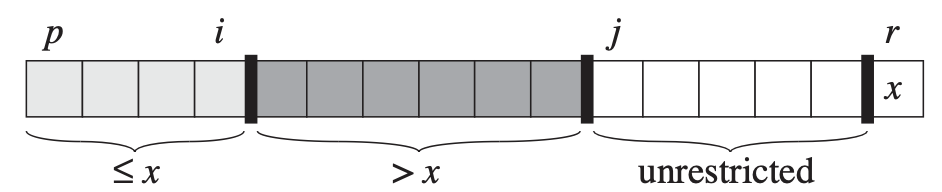
\includegraphics[width=0.7\textwidth]{assets/quicksort_areas.png}
    \caption{Regions maintained by PARTITION  (\cite{cormen2022introduction})}
\end{figure}

\subsubsection*{Performance}

The running time of quicksort depends on whether the partitioning is balanced or
unbalanced, which in turn depends on which elements are used for partitioning.
If the partitioning is balanced, the algorithm runs asymptotically as fast as merge
sort. If the partitioning is unbalanced, however, it can run asymptotically as slowly
as insertion sort.

\begin{itemize}
    \item \textbf{Best case}: $\theta(n\log n)$ \newline In the most even possible split, PARTITION produces two subproblems, each of
    size no more than n=2, since one is of size bn=2cand one of size dn=2e 1. In this
    case, quicksort runs much faster. The recurrence for the running time is then
    \begin{center}
        $T(n) = 2T(n/2) + \theta(n)$
    \end{center}
    where we tolerate the sloppiness from ignoring the floor and ceiling and from sub-
    tracting 1.
    \item \textbf{Worst case}: $\theta(n^2)$ \newline
    The worst-case behavior for quicksort occurs when the partitioning routine pro-
    duces one subproblem with n 1 elements and one with 0 elements. Let us assume that this unbalanced partitioning arises
    in each recursive call. The partitioning costs $\theta (n)$ time. Since the recursive call
    on an array of size 0 just returns, T(0) = \theta(1), and the recurrence for the running
    time is
    \begin{center}
        $T(n) = T(n-1) + \theta(n)$
    \end{center}
    \begin{figure}[H]
        \centering
        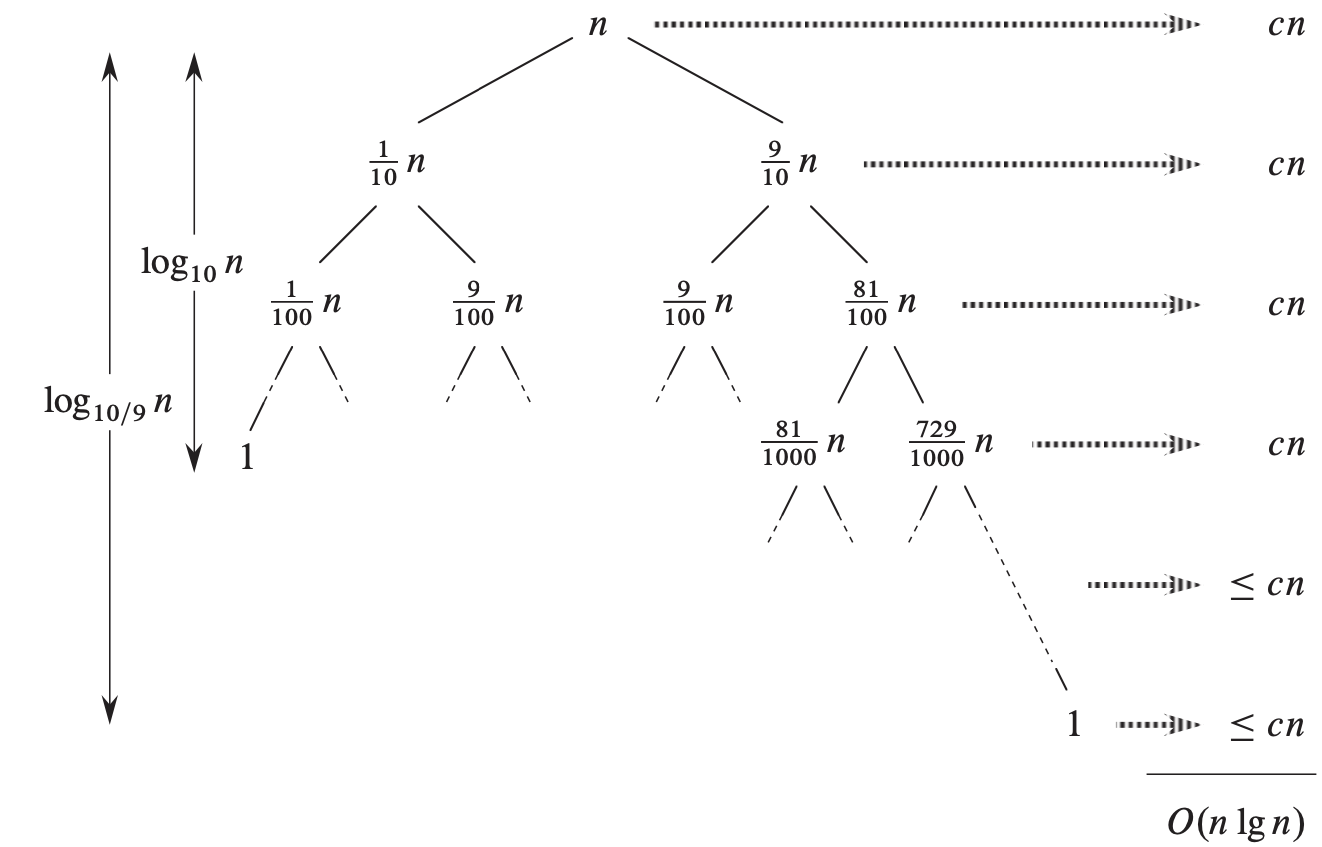
\includegraphics[width=0.7\textwidth]{assets/quicksort_avg_case.png}
        \caption{PARTITION always of 9 to 1 (\cite{cormen2022introduction})}
    \end{figure}
    \item \textbf{Average case}: $\theta(n\log n)$ \newline 
    When we run quicksort on a random input array, the partitioning is highly un-
    likely to happen in the same way at every level, we expect that some of the splits will be reasonably well balanced and
    that some will be fairly unbalanced. The average-case running time of quicksort is much closer to the best case than to the worst case.
    The total cost of quicksort is therefore $O(n\log n)$.
\end{itemize}

\subsubsection*{Characteristics}

\begin{itemize}
    \item \textbf{Stable}: No
    \item \textbf{In-place}: Yes
    \item \textbf{Online}: No
    \item \textbf{Divide and Conquer}: Yes
    \item \textbf{Parallelism}: Yes
    \item \textbf{Recursive vs Iterative}: Recursive
    \item \textbf{Space Complexity}: O($\log n$)
    \item \textbf{Comparison-based}: Yes
\end{itemize}






\section{Sorting in Linear Time}

Algorithms that can run on $\omega(n \log n)$ time complexity are considered to be linear time sorting algorithms. They share the property of determining the order of elements only by comparing them. For this they are called \textbf{comparison sorts}.

In a comparison sort, we use only comparisons between elements to gain order 
information about an input sequence $\langle a_1, a_2, \dots, a_n \rangle$. That is, given two elements 
$a_i$ and $a_j$, we perform one of the tests $a_i < a_j$, $a_i \leq a_j$, $a_i = a_j$, 
$a_i \geq a_j$, or $a_i > a_j$ to determine their relative order.

\begin{figure}[H]
    \centering
    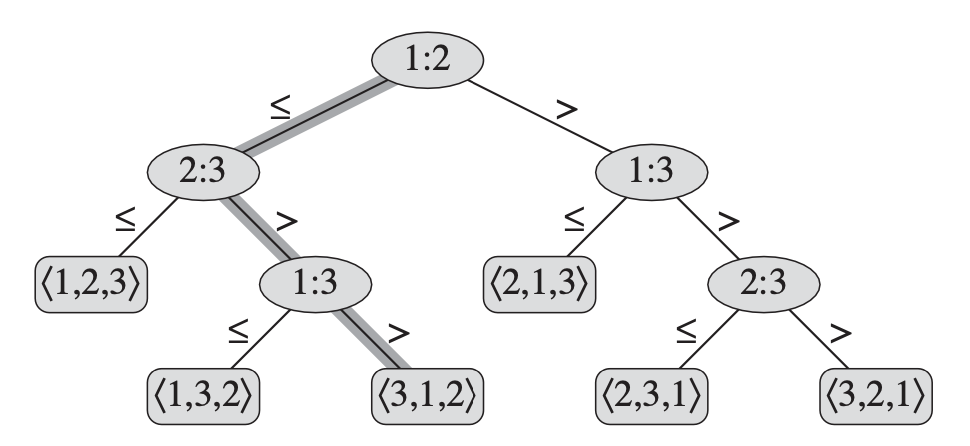
\includegraphics[width=0.7\textwidth]{assets/tree_model.png}
    \caption{Decision Tree Model (\cite{cormen2022introduction})}
\end{figure}

\definitionblock[Decision Tree Model]{The decision tree model is a way to analyze comparison-based sorting algorithms. In this model, the algorithm is viewed as a binary tree, where each internal node represents a comparison between two elements, and each leaf represents a permutation of the input. The height of the tree represents the worst-case running time of the algorithm.}

The length of the longest simple path from the root of a decision tree to any of
its reachable leaves represents the worst-case number of comparisons that the cor-
responding sorting algorithm performs. Consequently, the worst-case number of
comparisons for a given comparison sort algorithm equals the height of its decision
tree. A lower bound on the heights of all decision trees in which each permutation
appears as a reachable leaf is therefore a lower bound on the running time of any
comparison sort algorithm. 

\newtheorem{theorem}{Theorem}[section]
\begin{theorem}
    Any comparison sort algorithm requires $\Omega(n \log n)$ comparisons in the worst case.
\end{theorem}

\begin{proof}
    There are n! permutations of n elements, and any comparison sort algorithm must be able to distinguish among them to sort correctly. We can use a decision tree to model the algorithm. Each internal node of the tree corresponds to a comparison between two elements, and each leaf corresponds to a permutation of the input. Since the algorithm must be able to distinguish among n! permutations, the decision tree must have at least n! leaves. A binary tree of height h can have at most $2^h$ leaves. Therefore, we must have $2^h \geq n!$, which implies that $h = \Omega(\log n!) = \Omega(n \log n)$.
\end{proof}

\newpage

\subsection{Counting Sort}

Counting sort determines, for each input element x, the number of elements less
than x. It uses this information to place element x directly into its position in the
output array. For example, if 17 elements are less than x, then x belongs in output
position 18. We must modify this scheme slightly to handle the situation in which
several elements have the same value, since we do not want to put them all in the
same position.

In the code for counting sort, we assume that the input is an array $A[1,\dots,n]$ , and
thus A:lengthDn. We require two other arrays: the array $B[1,\dots,n]$ holds the
sorted output, and the array $C[1,\dots,k]$ provides temporary working storage.

\begin{figure}[H]
    \centering
    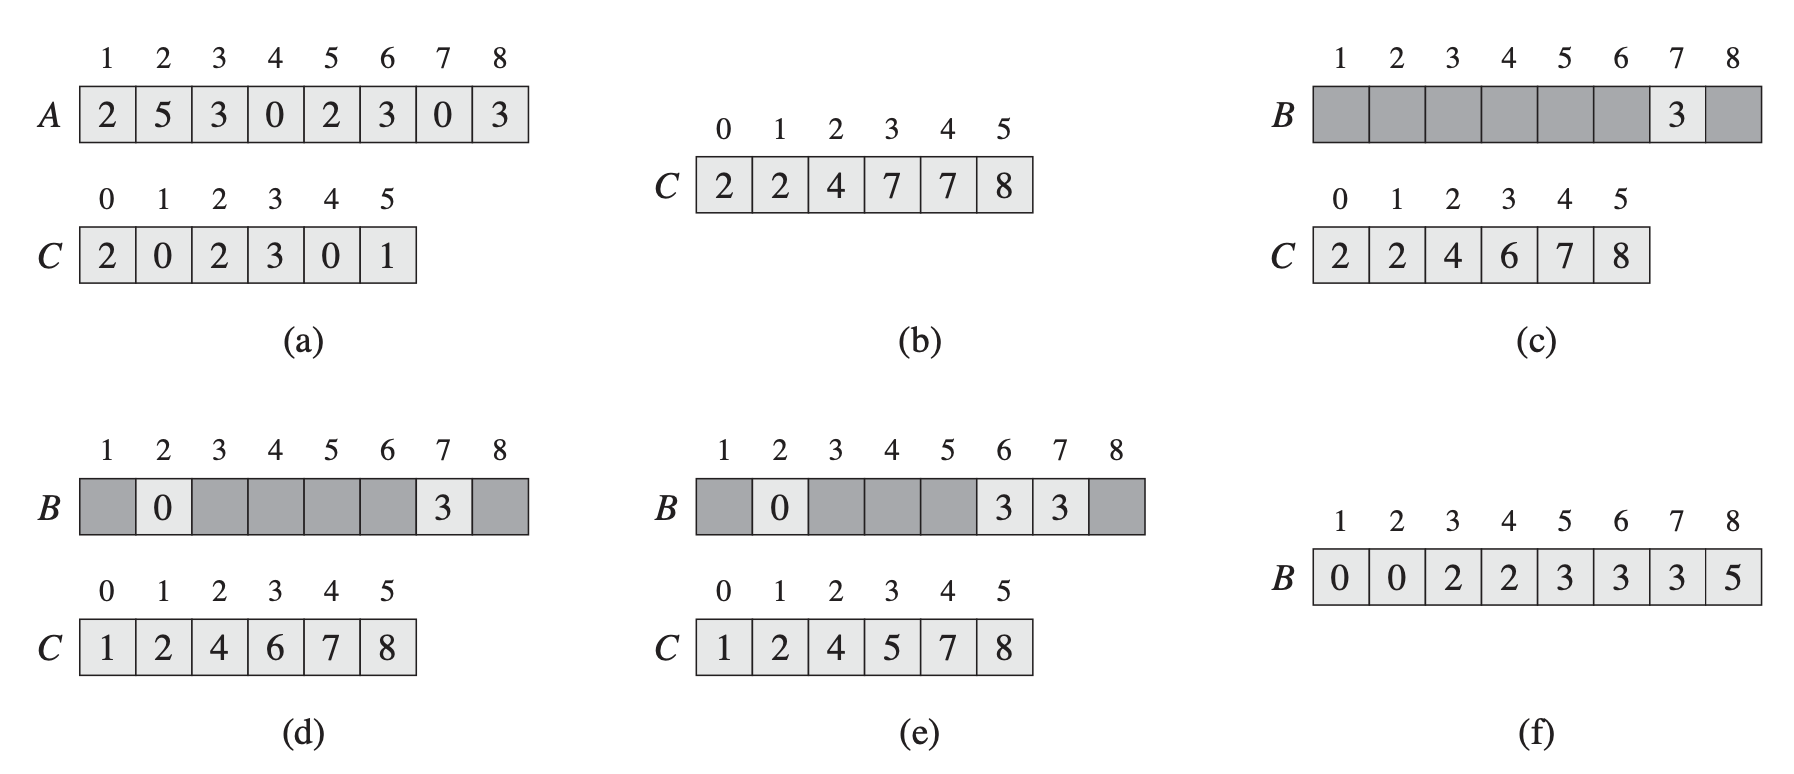
\includegraphics[width=0.9\textwidth]{assets/countingsort.png}
    \caption{Counting Sort (\cite{cormen2022introduction})}
\end{figure}

\begin{algorithm}[H]
    \caption{Counting Sort (A, B, k)}
    \For{i=1 to k}{
        C[i] = 0\;
    }
    \For{j=1 to A.length}{
        C[A[j]] = C[A[j]] + 1\;
        \tcc*{C[i] now contains the number of elements equal to i}
    }
    \For{i=2 to k}{
        C[i] = C[i] + C[i-1]\;
        \tcc*{C[i] now contains the number of elements less than or equal to i}
    }
    \For{j=A.length downto 1}{
        B[C[A[j]]] = A[j]\;
        C[A[j]] = C[A[j]] - 1\;
    }
    \tcc{Time complexity: $\theta(n+k)$}
    \tcc{Thus, the time complexity is $\theta(n)$ if $k = O(n)$}
\end{algorithm}

\observationblock[k]{
    \textbf{Counting sort} assumes that each of the n input elements is an integer in the range
    0 to k, for some integer k. When $k = O(n)$, the sort runs in $\theta(n)$ time.
}

The array B holds the sorted output, and the array C is used for temporary working storage for the number of elements encountered. 

An important property of counting sort is that it is \textbf{stable}: numbers with the same
value appear in the output array in the same order as they do in the input array. That
is, it breaks ties between two numbers by the rule that whichever number appears
first in the input array appears first in the output array. Normally, the property of
stability is important only when satellite data are carried around with the element
being sorted. Counting sort’s stability is important for another reason: counting
sort is often used as a subroutine in radix sort. For radix sort to work correctly, counting sort must be stable.

\subsubsection*{Characteristics}

\begin{itemize}
    \item \textbf{Stable}: Yes
    \item \textbf{In-place}: No
    \item \textbf{Online}: No
    \item \textbf{Divide and Conquer}: No
    \item \textbf{Parallelism}: No
    \item \textbf{Recursive vs Iterative}: Iterative
    \item \textbf{Space Complexity}: O(n + k)
    \item \textbf{Comparison-based}: No
\end{itemize}

\subsection{Radix Sort}

Radix sort is a non-comparison-based sorting algorithm that sorts integers by grouping them by individual digits. The idea is to sort the input numbers by their least significant digit, then by the next least significant digit, and so on, until the most significant digit. When k in in the range $1 \leq k \leq d$, where d is the number of digits in the input numbers, the time complexity of radix sort is $\theta(n)$.
Intuitively, radix sort breaks down each input integer into "columns" when they are written in some base b. Here d is the number of columns, and each column is a digit in the base-b representation of the number.In order for radix sort to work correctly, the digit sorts must be \textbf{stable}.

\begin{figure}[H]
    \centering
    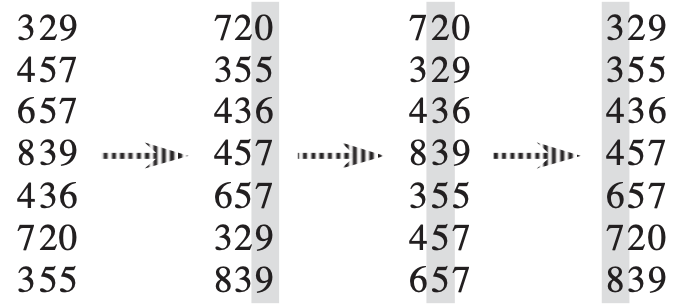
\includegraphics[width=0.7\textwidth]{assets/radixsort.png}
    \caption{Radix Sort (\cite{cormen2022introduction})}
\end{figure}

\begin{algorithm}
    \caption{Radix Sort (A, d)}
    \For{i=1 to d}{
        Use a stable sort to sort array A on digit i\;
    }
    \tcc{Time complexity: $\theta(d(n+k))$}
\end{algorithm}
\newpage
\newtheorem{Lemma}{Lemma}
\begin{Lemma}
    Given n d-digit numbers in which each digit can take on up to k possible values,
    RADIX-SORT correctly sorts these numbers in $\theta(d(n+k))$ time if the stable sort
    it uses takes $\theta(n+k)$ time.\end{Lemma}
\begin{proof}
    The analysis of the running time depends on the stable
    sort used as the intermediate sorting algorithm. When each digit is in the range 0
    to k 1 (so that it can take on k possible values), and k is not too large, counting sort
    is the obvious choice. Each pass over n d-digit numbers then takes time $\theta(n+k)$.
    There are d passes, and so the total time for radix sort is $\theta(d(n+k))$.
\end{proof}

\subsubsection*{Characteristics}

\begin{itemize}
    \item \textbf{Stable}: Yes
    \item \textbf{In-place}: No
    \item \textbf{Online}: No
    \item \textbf{Divide and Conquer}: No
    \item \textbf{Parallelism}: No
    \item \textbf{Recursive vs Iterative}: Iterative
    \item \textbf{Space Complexity}: O(n + k)
    \item \textbf{Comparison-based}: No 
\end{itemize}

